\documentclass[a4paper,10pt]{article}
\usepackage[utf8]{inputenc}
\usepackage{graphicx}
\usepackage{url}
\usepackage{float}
\usepackage{times}
\usepackage{multirow}
\usepackage{listings}
\usepackage{times}
\usepackage{paralist}
\usepackage{epsfig}
\usepackage{subfigure}
\usepackage[hypertex]{hyperref}
\usepackage{subfigure}
\usepackage{color}
\usepackage{xspace}

%\documentclass{rspublic}

\usepackage{ifpdf}

\newcommand{\I}[1]{\textit{#1}}
\newcommand{\B}[1]{\textbf{#1}}
\newcommand{\BI}[1]{\textbf{\textit{#1}}}
\newcommand{\T}[1]{\texttt{#1}}

\newcommand{\sagaspec}{\textit{SAGA}\xspace}
\newcommand{\sagaimpl}{\textit{SAGA}\xspace}

\newcommand{\spec}{\sagaspec}
\newcommand{\impl}{\sagaimpl}

\setlength\topmargin{0in}
\setlength\headheight{0in}
\setlength\headsep{0in}
\setlength\textheight{9.5in}
\setlength\textwidth{6.5in}
\setlength\oddsidemargin{0in}
\setlength\evensidemargin{0in}
\setlength\parindent{0.1in}
\setlength\parskip{0.25em}


\ifpdf
 \DeclareGraphicsExtensions{.pdf, .jpg}
\else
 \DeclareGraphicsExtensions{.eps, .ps}
\fi

\newcommand{\note}[1]{ {\textcolor{red} { ***NOTE: #1 }}}

\begin{document}

 \title{  \vspace{-3.5em}	SAGA AHM 2010 - Needs Title}
 
 \author{Shantenu Jha$^{1,2,3}$, Hartmut Kaiser$^{1}$, Andre Merzky$^{1}$, Ole Weidner$^{1}$ \\
   \small{\emph{$^{1}$Center for Computation \& Technology, Louisiana State University, USA}}\\
   \small{\emph{$^{2}$Department of Computer Science, Louisiana State University, USA}}\\
   \small{\emph{$^{3}$e-Science Institute, University of Edinburgh, UK}}
 }
 \date{}
 \maketitle
 

\subsection*{A Powerful, Community-Driven Standard}
A set of application groups conceived of the need and role for the
API, by expressing the desire for a simple programmatic interface that
would be widely-adopted and widely-available.  The goal of such an
interface is to provide a ``distributed computing counterpart to MPI''
(at least in impact, if not in details), and to supply developers with
a simple, uniform, and standard programmatic interface with which to
develop applications.  Thanks to the efforts of many contributors, but
in particular the efforts of the PI's group, an initial specification
of such an interface was released in 2008: the Simple API for Grid
Applications (\spec)~\cite{ogf-gfd-90}. The scope and requirements of
the \spec API have been formally defined by OGF's \spec Research Group
(SAGA-RG).  The SAGA-RG collected use cases from a broad user
community and published them as GFD.70 \cite{ogf-gfd-70}. The
requirements and design for the \spec API were directly derived from
these use cases; this process has been documented and published in
GFD.71 \cite{ogf-gfd-71}. The end result of this process is the 1.0
version of the \spec core specification (GFD.90 \cite{ogf-gfd-90}),
which defines language-independent syntax and semantics for the SAGA
core API (error handling, session and context management, permissions,
monitoring, attribute and task model) and functional packages (jobs,
name-spaces, files, replicas, streams, rpc). Several API extension,
such as CPR (GWD-R.96~\cite{ogf-gwd-r-96}), Adverts
(GFD-R-P.XX~\cite{ogf-gwd-r-p-xx}), and Messages
(GWD-R.94~\cite{ogf-gwd-r-94}) are currently under development and
follow a similar, well-defined community-driven standardization and
approval process. SAGA is now an Open Grid Forum (OGF)~\cite{ogf}
proposed recommendation on the path to becoming a standard.  The
standardization is not important in and of itself, but rather because
it makes it more likely that other infrastructures will also support
SAGA, which makes it, in essence, a de facto standard for users of
most national CI projects.

\subsection*{A Modular and Extensible Architecture}

The \impl \I{Core Components} and \I{Adaptors} an implementation
of the \spec API Specification written in C++ and Python. \impl is
Open Source software, released under the Boost Software
License 1.0~\cite{boost_license_web}. It can be divided into
three major components (as depicted in Fig. \ref{fig:saga_arch}):
the \I{Core Components} which provide the API functionality, the
\I{Adaptors} which translate API calls into native middleware calls,
the Python API \I{Language Bindings} and a set of \I{Command Line
  Tools}. The \impl \I{Core Components} are a collection of dynamic
libraries and header files that represent the functional API packages
(see section 2.1) along with a lightweight, highly-configurable
\I{Engine Component} that manages call dispatching and the dynamic
runtime loading of the \I{Middleware Adaptors}.


Each of these \I{Adaptors} implements the functionality of a specific
functional package (e.g., job adaptors, file adaptors) for a specific
middleware system. Adaptors are also realized as dynamic
libraries. \impl provides adaptors for many grid and distributed
computing middleware, including the Globus Toolkit, Condor, Platform
LSF and Amazon EC2. Several other adaptors, notably adaptors for PBS,
gLite and BES are under development. The Python API \I{Language
  Bindings} are an optional component of \impl that adds a thin Python
layer on top of the native C++ API. This simple but very popular
component allows application developers to quickly prototype and
implement \impl-based applications in Python.  The layered, decoupled
architecture of \impl allows for maximum flexibility at compile and
runtime. It allows the user of to freely and selectively combine the
library components and easily develop additional components orthogonal
to the existing ones. More details on \impl's architecture and its
implementation details can be found in \cite{OOPSLA_PAPER}.

%  The forth and last
% component are the \I{Command Line Tools}. They provide a
% non-programmatic access to each of \impl's functional packages: the
% \I{file tool} provides access to file operations, like read, copy,
% delete, move, etc., the \textit{job tool} allows simple submission and
% control ofcompute jobs, and so on.


\subsection*{A Mature Software Engineering Process\label{engineering}}

The \impl engineering process is closely supervised by the technical project manager. It follows an iterative and incremental model in which the evaluation and learning phase is strongly community driven. \impl provides independent releases for the \I{Core Components}, the \I{Language Bindings} and the \I{Adaptors}, which provides maximum flexibility and short shortest reaction times for bugfix-releases. All releases are available on the saga website~\cite{saga_downloads_web} and are fed into a very responsive community of users, which subsequently files bugs and suggests improvement through a central ticket system~\cite{saga_bugtracking_web} which is tightly integrated into the development process. These reports along with strategic long-term development goals form the requirements for the next iteration. Individual developers are usually responsible for specific components over the component's whole lifetime. This does not only ensure clearly defined targets for task assignments, but also results in growing expertise and specialization for the individual developers. The core \impl development team has been working together for more than three years and has evolved into a very smooth running operation. Nevertheless, the \impl development process is completely open: community involvement is not only accepted but encouraged and has lead to successful collaborations and enrichment of the \impl landscape in the past.

Along with the development of \impl, we maintain and constantly extend a broad set of unit and conformance tests to verify proper functioning and to validate OGF standard compliance. Most of the tests are written on a per-package basis using the Boost Test library~\cite{boost_test_web} and Python's built-in unit test framework. To facilitate the continuous integration (CI) aspect in the \impl development process, all tests are run constantly and automated using an automated CI rig\cite{buildbot_web} which provides feedback for every single change in the saga source tree. This way build problems and failing tests are pinpointed quickly and the responsible developer can take action. These automated tests are  our most valuable tool for early error and bug detection and has lead to a constantly higher quality of our releases since its introduction.
 
\subsection*{A Strong and Diverse Application Community}
\BI{Shantenu's playground}: talk about scientific applications using saga directly (...), talk about CS people taking saga and use it to build higher-level frameworks and tools (faust, bigjob, diggedag...). The usual stuff ;-)
 
 \pagebreak
 

\begin{figure}[hb]
  \centering
  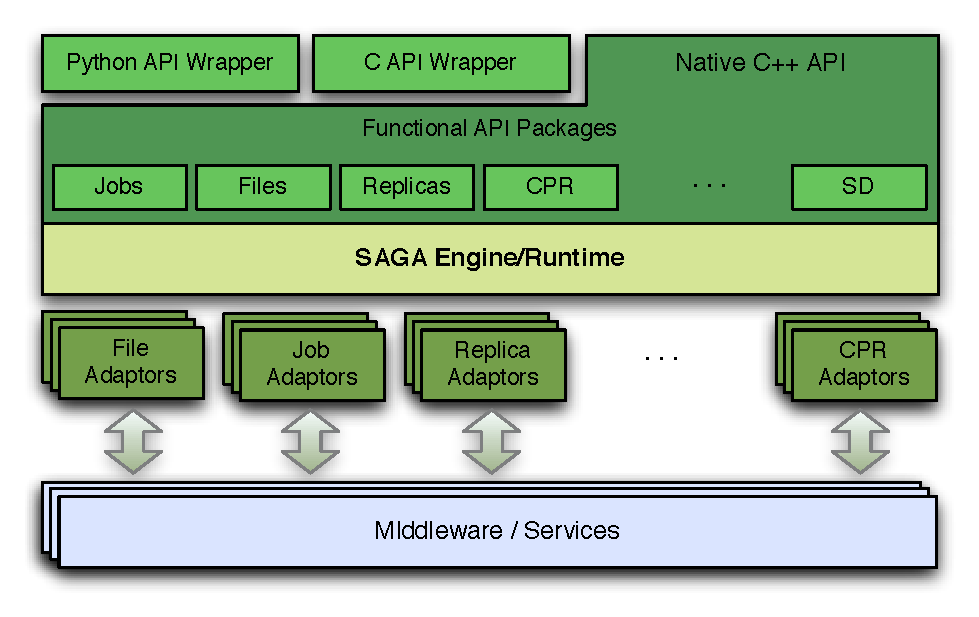
\includegraphics[width=4in]{./figures/figure_01}
 \vspace{-1em}	
  \caption{\footnotesize Layered schematic of the different
    components of \impl.  Middleware specific adaptors make
    applications developed using \impl portable.  Schematic showing
    the different ways in which \impl can be used to develop
    distributed applications. (i) Using native \impl calls to
    implement distributed functionality; (ii) Through the use of
    frameworks which provide either application-level usage modes,
    patterns and thus shielding the application from directly
    interfacing with the infrastructure.}
%\vspace{-1.5em}
  \label{fig:saga_arch}
\end{figure}

 \bibliographystyle{IEEEtran} 
 \bibliography{saga_ahm_abstract}


\end{document}

